\documentclass[letterpaper,12pt,preprint]{aastex}

% packages
\usepackage{amssymb,amsmath}

\newcommand{\project}[1]{\textsl{#1}}
\newcommand{\gaia}{\project{Gaia}}
\newcommand{\spitzer}{\project{Spitzer}}
\newcommand{\rewinder}{\emph{Rewinder}}

\begin{document}

\title{Inferring the Gravitational Potential of the Milky Way}
\author{Adrian M. Price-Whelan}

\section{Introduction}

Early large-scale, cosmological simulations of galaxy formation in the $\Lambda$CDM paradigm suggested that the spherically-averaged density profiles of dark matter halos follow a universal profile across a large dynamic range in mass \citep{navarro96}. Since then, higher resolution simulations --- both with and without baryons --- have produced dark matter halos that (1) are permeated with substructure on many scales, (2) are triaxial in shape, and (3) have shapes and orientations that vary with radius \citep{dubinski91, jing02, kuhlen07, veraciro11}. Dark-matter-only simulations produce triaxial halos \citep{jing02} with large density fluctuations \citep{zemp09}. Inclusion of baryons tends to soften the triaxiality and graininess in the inner galaxy through a combination of dissipative infall \citep{dubinski94} or cooling \citep{bryan13}. These processes combined with the gravity from a baryonic disk or ellipsoid can act to make the inner halo more oblate or spherical, however they do not seem to erase the clumpy, triaxial nature of the outer halo \citep[e.g.,][]{pontzen12}. This can lead to radially-dependent axis ratios, orientation, and smoothness, and suggests that the true mass distributions around Milky Way-like galaxies are not easily represented by simple potentials. Methods that seek to measure the potential of the Milky Way must be flexible enough to handle generic potentials where finding simple analytic forms or computing actions may not be possible.

The Milky Way affords us a three-dimensional view of the distribution of stars within in our own dark matter halo. Our proximity allows us to use individual stars as kinematic tracers and hence build much larger samples that probe deeper into the halo than the globular cluster and planetary nebula studies of external galaxies. Large photometric surveys such as the SDSS and 2MASS \citep{skrutskie06} have discovered a great deal of substructure in kinematic associations and streams of stars in the Milky Way halo \citep[e.g.,][]{belokurov06, rochapinto04}. Tidal streams are dynamically cold systems --- debris typically have small distributions of energy and angular momentum --- and thus require orders of magnitude fewer tracers than a random sample to get constraints of comparable accuracy to Jeans analysis. For example, in the simplest case we might assume that debris stars are actually still on the same orbit as their progenitor system \citep[a \emph{wrong} assumption, see e.g.,][]{eyre11}. This information about the orbits combined with measurements of the full-space velocities ${\bf v}$ at different points ${\bf x}$ in the structure (e.g., along a stream) would give us a direct measure of differences in a potential, $\Phi$.

\citet[][LM10]{law10} used N-body simulations of the disruption of the Sgr dwarf galaxy to simultaneously fit a model to the available data on the debris stars and a triaxial, analytic Milky Way potential. By varying parameters of the Milky Way potential, they found ``best-fit'' parameters by comparing the properties of observed Sgr stars to their simulated debris. The computational costs of running N-body simulations limited their search to a grid of potential parameters and forced the authors to fix many other parameters (e.g., properties of the disk and bulge). Nevertheless, they were able to constrain the 3D shape of the Milky Way potential out to $\sim$70 kpc and found that the best-fitting halo has a prolate, triaxial shape elongated in the Galactic Z direction, orthogonal to the plane of the disk. Though an unlikely orientation for the halo --- \cite{debattista13} find that the disk of the Milky Way would not remain stable in such a configuration --- LM10 showed that the data is at a state where such inference can be attempted. 

The computational costs associated with N-body simulations has motivated the development of many methods that approximately model tidal streams. The simplest alternative is to fit a single orbit to observed debris \citep[e.g.,][]{koposov10, deg13}. Though this is known to be incorrect and leads to biases in inferred properties of the underlying potential \citep[e.g.,][]{eyre11, lux13, sanders13a}, \cite{deg14} and \cite{lux13} have used orbit fitting to demonstrate the power of combining multiple streams in dynamical inference. To account for the offset between the orbit of the progenitor and the orbits of the debris stars, methods have been proposed that add some dispersion or offset around a single orbit either in phase space \citep[e.g.,][]{eyre09a, varghese11, kuepper12} or action-angle coordinates \citep{eyre11, sanders13b, bovy14, sanders14}. 

This thesis aims to (1) develop and test a probabilistic method for inferring the gravitational potential of the Milky Way using tidal streams, (2) apply this algorithm to real data (current data and a sample of stars with precise distances from our \spitzer\ survey of RR Lyrae stars), (3) explore the possibility of chaotic or highly non-linear dynamics within the Milky Way halo, and (4) study the process of satellite disruption in non-trivial Galactic potentials.

\section{Current/in progress: developing a method to measure the potential}
We are now in an era where full 6D information has been measured for stars in the halo. The quality of the data is often divided such that the on-sky position and radial velocity are precisely known but distance and proper motion components are only poorly constrained (and for many stars proper motions have not been measured). However, within the next year we will have precise ($\sim$2\%) distance measurements to a sample of RR Lyrae-type stars within the Sagittarius and Orphan streams, and, within a few years, \emph{tangential} velocities to the same stars with errors around $\sim$10 km/s from the \gaia\ mission. We focus on RR Lyraes because they, like Cepheids, exhibit a period-luminosity (PL) relation that enables precise distance measurements to individual stars (see Section~\ref{sec:smash}).

Motivated by the prospect of future, 6D information for individual stream stars, \cite{johnston99a} proposed a simple method for using such stars to measure the underlying gravitational potential of the Milky Way's halo based on the fact that stars observed in a stream must have been disrupted from a progenitor at some time in the past. Given present-day positions and velocities for stars in a stellar stream, and the present-day position and velocity of the progenitor of the stream, the orbits of the stars and progenitor were integrated backwards, and the best potential was the one in which the most stars were ``recaptured'' by the progenitor (based on a threshold in relative energy). Put another way, to find the best-fit potential parameters, \cite{johnston99a} maximized the number of stars recaptured by the progenitor for a given choice of potential parameters.

In \cite{apw13} we revisited this idea, but rather than counting stars that are captured, we studied the distribution of debris star orbits as the stars are disrupted using a ``phase-space distance''
\begin{equation}
	D_{\rm ps} = \sqrt{\frac{\vert{\boldsymbol{x} - \boldsymbol{x}_{\rm p}\vert^2}}{r^2_{\rm tide}} + 
				    \frac{\vert{\boldsymbol{v} - \boldsymbol{v}_{\rm p}\vert^2}}{v^2_{\rm esc}}}
\end{equation}
where $(\boldsymbol{x},\boldsymbol{v})$ and $(\boldsymbol{x}_{\rm p},\boldsymbol{v}_{\rm p})$ are the positions and velocities of star and progenitor, respectively, and $r_{\rm tide}, v_{\rm esc}$ are the tidal radius and escape velocity. We integrated the star orbits backwards to find the minimum phase-space distance for each star and minimized the variance of the distribution of minimum phase-space distances. We found that with a sample of $\sim$100 stream stars from a Sgr-like stream, we are able to constrain properties of a multi-component Galactic potential model with a triaxial, logarithmic halo. This idea, \rewinder, while closer to modeling the stream debris, will only work when 6D phase-space information is known for stars and progenitor, and does not properly account for the uncertainties on the measurements.

We have since identified a minimum set of issues that any approximate stream model or potential recovery method should address:
\begin{enumerate}
	\item \textbf{Observational uncertainties:} The known debris structures are $\gtrsim$10 kpc from the Sun, where distance and proper motion measurement errors are significant. Thus it is critical for any method that uses tidal debris to incorporate observational uncertainties and missing dimensions in a consistent and justified way. 
	\item \textbf{Form of the potential:} There is large uncertainty in the radial profile, shape, orientation, and graininess of the outer halo and the constancy of these parameters over distance. Properly describing the potential may require non-parametric techniques or complex analytic functions so the method should not rely on the existence of or ability to compute simple conserved orbital properties, such as actions.
	\item \textbf{Multiple debris structures:} Near-future photometric surveys such as \gaia\, and the \project{LSST} will likely discover many new streams and kinematic associations of stars. Potential recovery methods should be able to simultaneously use multiple streams and incorporate other dynamical constraints.
	\item \textbf{Comparing models to data:} Matching generated streams to observed stellar densities is difficult; models that rely on this must account for observational biases, internal properties of the progenitor, and background halo stars.
	\item \textbf{Computational expense:} Full N-body simulations are expensive to run; incorporating an N-body simulation into a likelihood function evaluation and then performing a parameter search would be computationally intensive and, presently, intractable. 
\end{enumerate}

Our current work (also attached; Price-Whelan et al. (in prep.)) formalizes \rewinder\ by defining a proper likelihood function based on the simple method of \cite{apw13} and addresses each of the above points. By analyzing a suite of N-body simulations over a range of progenitor masses on the same orbit, we find that even in a triaxial halo potential the debris disrupts through instantaneous Lagrange points with some dispersion related only to the mass ratio of the progenitor to the enclosed mass of the parent potential and the orbit of the progenitor (see Figure~\ref{fig:lpts_r}, same as Figure~3 in the paper draft). This motivates a model for tidal debris in which each star was ``released'' at the instantaneous, effective Lagrange point at its unbinding time with a dispersion in position and velocity, all of which depend only on the mass and orbit of the progenitor and the parent potential.

\begin{figure}[h]
\begin{center}
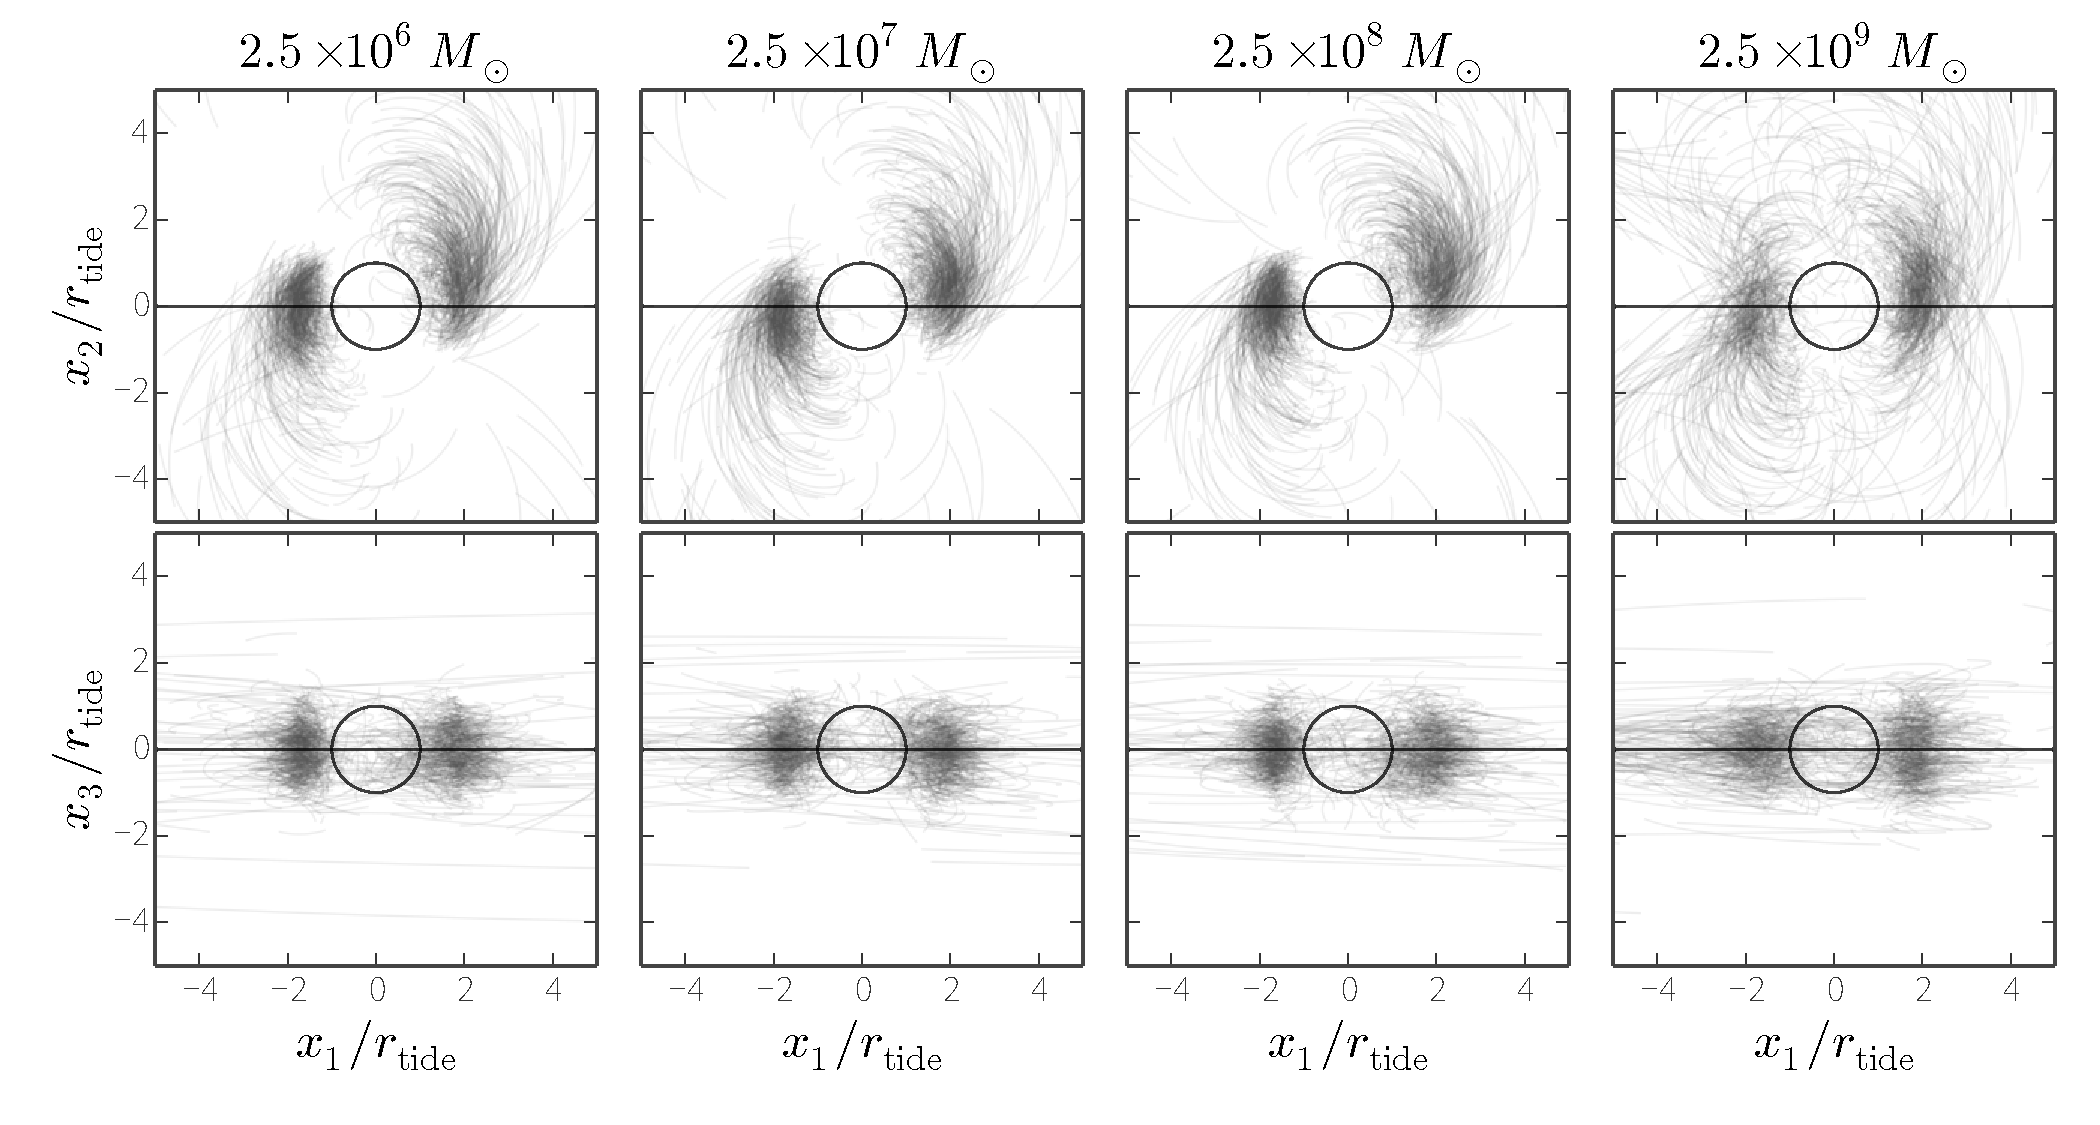
\includegraphics[width=\textwidth]{../../streams/plots/paper2/Lpts_r.png}
\caption{ Orbits of 2000 randomly drawn particles projected into instantaneous orbital plane coordinates (Eqs.~11-13 in the paper draft), normalized by the tidal radius, and only shown within half a satellite crossing time around their unbinding time for each of four progenitor masses. The orbits were integrated backwards from their present-day positions (final time step of the N-body simulations) as test particles without the potential of the progenitor. Horizontal black line shows $x_2=0$ (top panels) and $x_3=0$ (bottom panels), and the unit circle (black circle) shows the classical disruption radius in these coordinates. }\label{fig:lpts_r}
\end{center}
\end{figure}

\rewinder\ handles observational uncertainties and missing data dimensions by including the true 6D positions of stars and the progenitor as model parameters. It works in ordinary phase-space and relies on direct orbit integration; we do not make any assumptions about the integrability or form of the potential. It can therefore support arbitrarily complex potential functions that contain, for example, basis function expansions or explicit time dependence. By expressing the model in terms of a likelihood function with priors on the parameters, incorporating multiple streams into the inference only requires multiplying the likelihoods computed for each stream and progenitor pair. Thus, handling multiple debris structures should be a trivial extension. We have performed several experiments on data of just four stars from a simulated stream with varied data quality to show that \rewinder\ simultaneously constrains the potential and models a tidal stream. For more details, see the attached paper draft. 

\section{Next steps: applying to real data}

Our goal is to provide precise measurements of the Milky Way potential using tidal streams by (1) developing a framework for using arbitrary potential models in the inference, (2) combining multiple streams and debris structures, and (3) using extremely precise distance information for RR Lyrae stars in the SMASH survey (see Section~\ref{sec:smash}). Measurements of the potential at this level of detail will hopefully begin to shed light on the global structure of dark matter around the Milky Way, better constrain the mass of the Galaxy, and provide constraints on the granularity or amount of substructure. Below I briefly outline the components of my research plan for the coming years.

Thus far we have only tested \rewinder\ on simulated observations of particles from N-body simulations. We have demonstrated in Price-Whelan et al. (in prep.) that we are able to use a small sample of stars (4) with realistic observational uncertainties to recover the parameters of the ``true'' potential used in the simulations. The immediate next step for this project is to apply \rewinder\ to real data that is available now for the Orphan stream. Before we do this we will have to use some tricks to lower the dimensionality of our parameter space to make the inference computationally tractable.

\subsection{Orphan stream with current data}

One shortcoming of \rewinder\ is that the number of model parameters scales with eight times the number of stars --- the six, true phase-space coordinates for the star, the tail (leading or trailing), and the time the star was disrupted from the progenitor are model parameters for each star. Properly modeling real data from the Orphan or Sagittarius stream (where we expect to have $\sim10-100$ well-measured RR Lyrae stars) with \rewinder\ would then require sampling over a parameter space with hundreds of free parameters. It is extremely difficult to sample from high dimensional probability functions; with a large number of parameters, it is almost guaranteed that there will be local optima that present challenges to most MCMC algorithms. Once our current paper is submitted, we will revisit the definition of the likelihood function and explore the idea of internally marginalizing over the coordinate parameters. This non-trivial technical improvement, if possible, would greatly reduce the number of free parameters and make the MCMC sampling much faster. 

Once we can run with a realistic sample of many 10's of stars, we will use current data for a sample of RR Lyraes in the Orphan stream which have measured radial velocities, photometric distances, and (poor) proper motions to constrain the present position of the progenitor of the stream, which is presently unknown. This would provide a direct target for observational campaigns to hunt for the Orphan progenitor, and simultaneously place constraints on the potential using a stream that is nearly orthogonal to the Sagittarius stream.

\subsection{SMASH RR Lyrae (near-future data)}\label{sec:smash}
The PL relation for Cepheids is prominent in optical passbands but for RR Lyrae stars the scatter in the PL relation is smallest at mid-infrared wavelengths. The IRAC instrument on the \spitzer\ Space Telescope was recently used to measure distances to several nearby RR Lyrae with HST proper motions and found that with the mid-infrared PL relation enables distance measurements to individual stars with 2\% errors \citep{benedict11, madore12}. The SMASH program is an accepted \spitzer\ Cycle 10 program (PI: K. V. Johnston) that will exploit this unprecedented opportunity to precisely map structures throughout the halo of our Galaxy. The program has been allotted all $\sim$650 hours of requested time and will proceed through 2014-2015. SMASH will construct the first 3-D map of the Sagittarius dwarf galaxy remnant, it will determine precise distances to four other satellites (Ursa Minor, Carina, Sculptor, \& Bootes), and make the only measurements of stars in the Orphan and Sagittarius streams accurate enough to determine their individual positions within the debris. 

As part of the SMASH team, I will lead the group on analyzing and interpreting the Sagittarius stream stars and play an active role in the modeling of the Orphan stream. We anticipate producing the best measurement of the Galactic potential to date, a groundbreaking achievement that will demonstrate the power of tidal streams as dynamical potentiometers.

\subsection{Future data}
The \gaia\, project will deliver hundreds of millions of stars useful for dynamical inference, but it might turn out that particular streams and stellar subsamples within those streams will be the most relevant for inferring the Milky Way potential. RR Lyrae stars can in principle deliver precise photometric distances at essentially all halo distances \citep{madore12}, but these stars are rare (and their abundances are age and metallicity dependent). There could be many cold structures in the Milky Way halo that are highly constraining on the potential, but which contain only a few good distance-indicating members. It is not yet known what the trade-offs are between having many stars at low precision and a few at high precision, nor is it known how valuable distance information really is when a structure contains many precisely observed members. 

An open question is which stars and kinematic data should we be focusing our observational efforts on? For example, precise distances might be more important for providing meaningful potential constraints for certain streams, where for other streams the velocities might be sufficient and necessary. Given the current status of the data for each stream, it would be extremely beneficial to know what data we need in order to improve measurements of the potential. We are equipped to answer these questions with \rewinder.

\section{Related dynamics / theoretical projects}
\subsection{Chaos in the Milky Way}
Many models for stream formation assume that the underlying gravitational potential is smooth and can be well-approximated by a (set of) integrable potentials --- that is, gravitational potentials that admit a sufficient number of constants of motion (in involution) to directly solve the equations of motion. It is often hard to determine whether a given potential is integrable, and one open question is whether any of the most realistic Galactic potentials (triaxial potentials with non-trivial radial dependence) would display chaos. 

A common check for chaotic behavior is to compute the Lyapunov exponent; two orbits separated by an infinitesimal offset $\delta \boldsymbol{x}_0$ at some initial time will diverge according to $\vert\delta \boldsymbol{x}(t)\vert \sim \vert\delta\boldsymbol{x}_0\vert e^{\lambda t}$, where $\lambda$ is the Lyapunov exponent. If $\lambda > 0$, this is an indication that the Hamiltonian admits chaos. Another way to think about this is through the Lyapunov time, which is simply $t_\lambda = \lambda^{-1}$. If the Lyapunov time is long (e.g., 10's of Gigayears), we wouldn't expect to see any signature of chaos within the Milky Way halo. However, if the Lyapunov time is comparable to the orbital time of an infalling satellite, chaos will act to ``truncate'' streams and debris structures. The presence of cold debris structures in the halo puts a lower limit on the Lyapunov time, however if it is somewhere in the middle, this would greatly effect any inferences that use tidal streams as potential measures.

\subsection{Disruption mechanisms}
In modeling the disrupted debris, we have assumed that it is steadily removed from the progenitor system via tidal pruning or gentle tidal forcing. Even on a mildly eccentric orbit, stars are preferentially stripped around the satellite's pericenter because of tidal shocking, but for a mildly eccentric case the shocking only acts to enhance the rate of disruption, not alter the distribution of debris as it becomes unbound from the progenitor. On more eccentric orbits, when tidal shocking dominates, the debris forms morphologically different shell or cloud-like structures. The distinction between stellar streams and stellar clouds is just related to the orbit of the disrupting satellite within the parent galaxy. By incorporating a prescription for tidal shocking in \rewinder, we could also apply it to shell-like structures such as the Triangulum-Andromeda \citep{rochapinto04} or Hercules-Aquila \citep{belokurov07b} stellar clouds.

\section{Timeline}
\noindent\begin{description}
	\item[Spring 2014] 
		\noindent\begin{itemize}
			\item finish paper presenting probabilistic model and submit (\rewinder)
			\item begin working on marginalizing over coordinate parameters
			\item background reading on chaos and nonlinear systems
		\end{itemize}
	\item[Summer 2014] 
		\noindent\begin{itemize}
			\item finish internal marginalization of coordinate parameters
			\item begin running tests on real data (Orphan stream)
			\item define project with H-W Rix at MPIA
			\item background reading on chaos and nonlinear systems
		\end{itemize}
	\item[Fall 2014] 
		\noindent\begin{itemize}
			\item write up paper on Orphan stream with current data
			\item begin running tests with SMASH data
			\item continue working on Rix project
			\item begin exploring implications of chaos within the Milky Way
		\end{itemize}
	\item[Winter 2014-2015] 
		\noindent\begin{itemize}
			\item write up paper on Orphan stream with current data
			\item run inference on SMASH data, begin writing Sagittarius paper
			\item continue working on Rix project
			\item continue working on chaos within the Milky Way
		\end{itemize}
	\item[2015+] 
		\noindent\begin{itemize}
			\item finish SMASH paper on inferring the potential with the Sagittarius stream
			\item finish Rix project
			\item finish chaos within the Milky Way project
			\item begin work on disruption mechanisms
			\item begin preparing for initial Gaia release
		\end{itemize}
\end{description}

\bibliographystyle{apj}
\bibliography{refs}

\end{document}
